\chapter{Architecture/Model}
\label{sec:architectureAndModel}
This chapter contains the architecture and model of the system, which tools and methods that has been used and how they all connect together to produce the result.
An overview of the system is presented in chapter \ref{sec:overview}. 
\begin{figure}[h]
\label{fig:overview}
\begin{center}
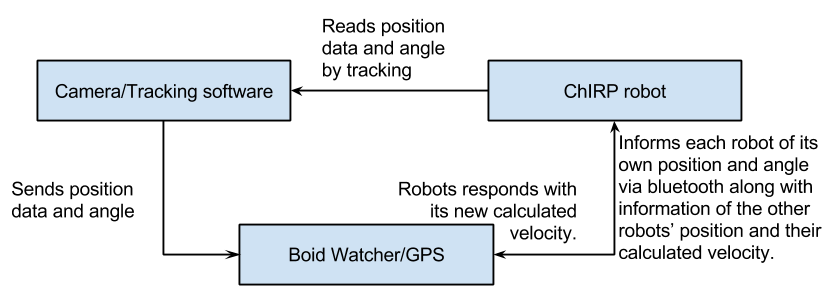
\includegraphics[width=0.8\linewidth]{figs/system_overview}
\end{center}
\end{figure}
\section{System overview}
\label{sec:overview}
The system consists of three primary components as illustrated in Figure \ref{fig:overview}. The camera and the tracking software, the Boid-watcher (simulator) software and the ChIRP robots.
The camera tracking software tracks each robot's position and its angle, which is sent to the Boid-watcher simulator. The Boid-watcher simulator is the bridge between the robots, it provides information about the position and velocity of each robot to each robot - it acts like a Global positioning system.
The camera tracking software being run on a stationary desktop computer, and the camera is attached to a pole above a sandbox where the robots roam around.
The simulator is run on a different computer, because it needs to communicate with all the robots simultaneously 
%TODO GPS

Robots
eight distance sensors, using only the three in front for collision detection
two wheels



Robot code


Here you will present the architecture or model that you have chosen and that is (or will be) implemented in your work. Note that putting algorithms in your report is not desirable but in certain cases these might be placed in the appendix. Code further be avoided in the report itself but may be delivered in the fashion requested by the supervisor or, in the case of masters delivery, submitted as additional documents. 